\section{Approach}
\label{sec:approach}

\begin{figure}[th]
\centering
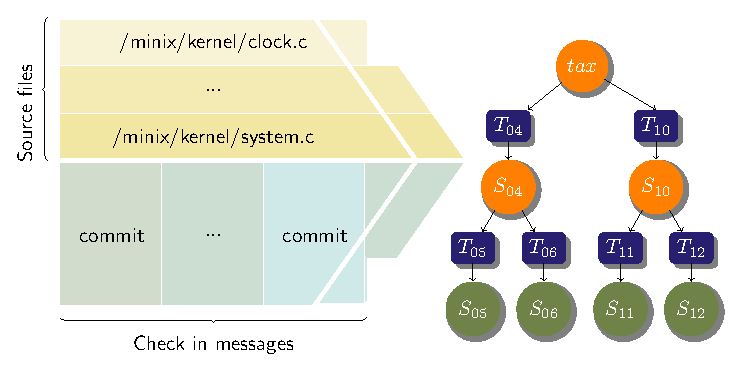
\includegraphics[width=0.6\columnwidth]{picture/framework.eps}
\caption{ICQ Workflow. \textcircled{1}: data filtering phase; \textcircled{2}: cue discovery phase; 
\textcircled{3}: model probing phase. $f$=a specific feature, $R$=training data, $S$=test data, $R_f$=filtered training data, 
$S_f$=filtered test data, $S_{nf}$=remaining test data without feature $f$, $\overline{S_f}$=flatten test data, $\mathcal{M}$=a sepecific model.}
\label{fig:framework}
\end{figure}

The ICQ framework is illustrated in~\figref{fig:framework}.
In the \textit{data filtering} phase, it extracts from the dataset
those problematical instances that contain a given linguistic feature $f$. 
In the \textit{cue discovery} phase, it identifies the possible cues among pre-defined features. 
Finally, in the \textit{model probing} phase,
it does two tests: ``accuracy test'' and ``distribution test''.
Next, we will discuss these phases in more detail.

%\KZ{The workflow
%here evaluates the ``cueness'' of one specific linguistic feature $f$ of a
%given data set which consists of a training set and a test set.
%We first filter the training set and the test set respectively into two
%subsets of instances that carry the given linguistic feature. We then
%compare the label distribution of these two subsets (blue and red). If 
%there is substantial similarity, then the dataset is declared to be
%inflicted with the cue on $f$. 
%We can modify the test subset into a {\em neutral
%test} set $ST$
%by duplicating cases with underrepresented labels and effectively
%flattening the red distribution \KZ{use some notations here and in the fig
%for easy narration.} Now, suppose we have a model $M$,
%trained from the original training data, and we apply $M$ on the $ST$, to make
%predication results. If the label distribution of these results
%(green distribution) is again similar 
%with the original training data distribution (blue), we can conclude
%that model $M$ does exploit the feature $f$ in its inference and its
%accuracy maybe over-estimated.  Next we explore several
%shallow linguistic features which act as possible cues, and 
%give details on how the dataset and the model can be evaluated against
%these features.}

%
%ICQ can be broken down into the following phases: feature definition, 
%dataset filtering and evaluation, and model evaluation. With ICQ, we 
%discover whether the data have spurious cues, and whether a model is 
%sensitive to a particular linguistic feature during inference.

%WeWe evaluate the information leak in the datasets by statistical cues only. 
%First, we formulate  a number of NL reasoning tasks in a general form. 
%Then based on the cues associated with each label, 
%we design a number of metrics to measure the correlation between words
%and labels. Such correlation scores are called ``cue scores'' because they are 
%indicative of potential cue patterns. Afterwards, we aggregate the scores 
%using a number of simple statistical
%models to make the predictions. Finally, we show how to split a dataset into
%the easy and hard parts using the above fast predictions.

\subsection{Data Filtering Phase}
\label{sec:evaldata}
%Given the features $F$,
Once we have defined the linguistic features, the fundamental step of our system 
can build a data filter for
each feature value $f$. 
A filter takes a dataset and returns
a cluster of instances associated with that feature value. For example,
there is a filter for the word ``happy'' in ROCStories task,
and we can get all the instances that 
contains the word ``happy'' in their endings including Example \ref{exp:roc}. 
Similarly, there are filters for ``PER'' entity, ``negative'', ``sentiment'', etc. 


\subsection{Cue Discovery Phase}
\label{sec:cuenessdiscovery}
For each feature $f$, we apply its filter to both the training data and test data
of $X$, denoted as $R$ and $S$ in \figref{fig:framework},
resulting in a clustering subset of training instances and test instances 
that are defined as $R_f$ and $S_f$. 
It should be noted that only those features 
that appear both in the training and test data
are qualified as possible cues for a dataset.
Let $y_i$ be the number of instances with label $l_i$ in the filtered
dataset $F$, then we can compute the bias of the label distribution for a filtered
set by the mean squared error (MSE):
%\KZ{Fix the notation for MSE.}

\begin{equation}
MSE(F) = \frac{1}{|L|} \sum_i (y_i - \overline{y_i})^2
\end{equation}
where $\hat{y_i}$ is the mean of $y_i$. The larger $MSE(F)$, 
the more ``pointed'' the label distribution and more biased. 
Furthermore, if the filtered training set and 
the filtered test set are biased similarly,
the Jensen-Shannon Divergence(JSD)~\cite{lin1991divergence} between
the distribution of them is small:
\begin{equation}
JSD(R_f, S_f) = \frac{1}{2}\left (Q(R_f)\parallel A  \right )+\frac{1}{2}\left (Q(S_f)\parallel A  \right ), 
\end{equation}
where $ A = \frac{1}{2}\left (Q(R_f)+Q(S_f) \right )$. 
%\KZ{Complete the above formula.} 
$Q()$ denotes the label distribution of the filtered dataset.
Finally, we define a cueness score as
\begin{equation}
cue(f, X) = \frac{MSE(R_f)}{\exp(JSD(R_f), S_f))}
\end{equation} 
which represents how much a dataset $X$ 
is biased against a feature $f$. 

%\KZ{Add a comparison between this cue function and other possible cue functions
%such as PMI in eval. By computing the distance between the ranking induced by
%the cueness and the rankings by the four models $\Delta$.}

\subsection{Model Probing Phase}
\label{sec:modelprobing}

Following the previous section, 
we can illustrate that if a dataset $X$ is infected with a cue $f$. 
%from previous
%test in \secref{sec:evaldata}.
However, it doesn't mean
the model trained from this dataset necessarily exploits that cue. 
Because models are determined by both data and model architecture. 
If the model is strong enough, it won't be affected by data bias easily. 
Here we propose a simple framework to probe any model instance trained from the
given biased dataset~\footnote{Models trained from any other 
datasets compatible in format with $X$ can also be used to probe its potential
bias on the same cue.} to see if it actually takes advantage of that cue $f$
and by how much. We can do that through two simple tests: 
{\em accuracy test} and {\em distribution test}. 

\subsubsection{Accuracy Test}
\label{sec:accuracytest}

In the accuracy test, we simply assess the prediction accuracies of the model
$M$ on the filtered test set (with feature $f$) and on the remaining test (without feature $f$), 
and call them $acc(S_f)$ and $acc(S_{nf})$, respectively. 
The accuracy test shows the difference
between these two accuracies: 

\begin{equation}
\Delta Acc(f)=acc(S_f) - acc(S_{nf})
\end{equation} 

if the $\Delta Acc$ score is greater 0, then the
model is considered to be biased and to have exploited this cue. 
The value $\Delta$ measures the extent of the bias.


\subsubsection{Distribution Test}
\label{sec:distributiontest}
Distribution test is a visual test. We first create a ``stress data set'' $\overline{S_f}$
by ``flattening'' the label distribution in $S_f$.  
We achieve that by replicating random instances from all labels 
except the most popular label in the filtered test
set and adding them back into the set. 
The repetition augmentation procedure stops when 
the feature distribution based on each label is balanced.
This way we have effectively removed the bias 
in the filtered test set and presumably 
posed a challenge to the model. 
Next, we apply the same model to the stress test set 
to get prediction results. 
We compare the label distribution of the prediction results on 
the stress test set with the label distribution of 
the filtered training data.
The idea is, if the filtered training data contains a cue, 
its label distribution will be skewed toward a particular label.
If the model exploits this cue, it will prefer to predict
that label as much as possible, even amplifying the skewness
of the distribution, despite that the input test set has been
neutralized already. We hope to witness such amplification
in the output distribution to capture
the weakness in the model.

%If the two distributions are similar enough, 
%we deem the model biased toward that feature and not robust enough.
%This similarily can be displayed visually. 
The above two tests are related but not equivalent
and their outcomes complement and reinforce each other. 
If both tests conclude that the model is sensitive to a certain feature, 
then there is a high probability that this is the truth.

%but don't provide new method for data augmentation. 
%We require a more fair dataset to test if a model is sensitive to a feature. 
%The filtered test dataset of a feature in \figref{fig:framework} (red) is unbalanced among 
%labels. The number of cases for each label can be denoted as $c_{ent}, c_{neu}, c_{con}$~(in 
%SNLI task). If any of these number is smaller than a threshold $\sigma$, 
%we won't consider to test this feature, because
% this feature is not well supported by enough data. 
%%If the smallest number of samples among different labels is lower than 
%%a threshold $\sigma$, we won't consider to test this feature. Because
%% this feature is not well supported by enough data. 
%The smallest number can be denoted as $c_{min}=min(c_{ent}, c_{neu}, c_{con})$.
%To make the result more intuitive and fair, 
%we flatten the distribution by removing $c_{l} - c_{min}$ cases from 
%the filtered cases with label $l$ 
%resulting in the orange ``stress test'' 
%in \figref{fig:framework}. 
%Then we test the model on this stress test. 
%The similarity between prediction result (green) and 
%training data distribution (blue) on a feature indicates how the model 
%is influenced by the appearance of this feature in training data. 

%It is insufficient for testing if the filtered test data size is quite small or samples on 
%some label is rare which bellow a threshold $\sigma$. 
%Thought we can't generate cases for feature, we can point out what kind of 
%test samples should be augmented. 
%The similarity is 
%calculated by Kullback-Leibler (KL) Divergence.
